\section{Introduction}

World models and video planners give embodied agents a tempting interface: imagine futures, score them against a goal, and execute the best one. This interface is insufficient when the future is evaluated only as a passive visual sequence. A generated transition may be smooth, likely under video data, and goal-satisfying, while still being impossible for the current embodiment to realize in one local step. A nonholonomic car cannot move sideways without changing heading. A pusher cannot move an object before contact. An arm near a singular configuration cannot realize every Cartesian displacement within its action limits.

This paper studies the local test that is missing from such futures. Let $z_t$ be a representation state and let $J_\phi(z_t)$ map small controls into representation-space changes. The local action-reachable tangent set is
\[
\A(z_t)=\{J_\phi(z_t)u:u\in \U\}.
\]
For an imagined transition $\Delta z_t=z_{t+1}-z_t$, we define the actionability residual
\[
r_t=\min_{u_t\in \U}\left\|\Delta z_t-J_\phi(z_t)u_t\right\|_W^2+\lambda\|u_t\|^2.
\]
The score is small when the transition can be explained by a bounded local action and large when the generated future leaves the embodiment's reachable tangent set.

The idea is complementary to recent Jacobian-based robot policies and executable-video systems. Neural Jacobian Fields and VERA show that local visual Jacobians can translate desired visual change into action \citep{li2024jacobian,li2026vera}. EVA aligns video world models with inverse-dynamics rewards \citep{wang2026eva}. World Action Verifier asks whether world-model futures are executable through forward-inverse asymmetry \citep{liu2026wav}. Here we isolate a simpler representation-level question: before or during trajectory inference, can we certify that the local transition lies near the action tangent set of the current embodiment?

\paragraph{Contributions.}
First, we formalize an actionability residual for generated representation trajectories and connect it to local execution error. Second, we build a CPU-first benchmark with four toy embodiments that expose different non-executability modes. Third, we show that the residual predicts execution failure and supports repair when composed with world, goal, smoothness, and constraint energies. Fourth, we demonstrate embodiment swapping: the same imagined displacement can be feasible for one body and infeasible for another by changing only $J_\phi$.

\begin{figure}[t]
\centering
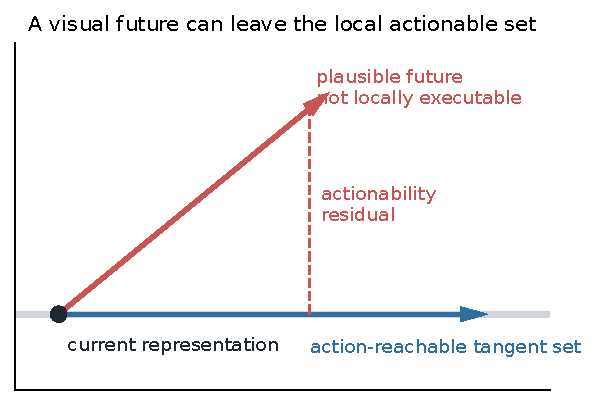
\includegraphics[width=0.45\linewidth]{figures/fig1_concept_actionability.pdf}
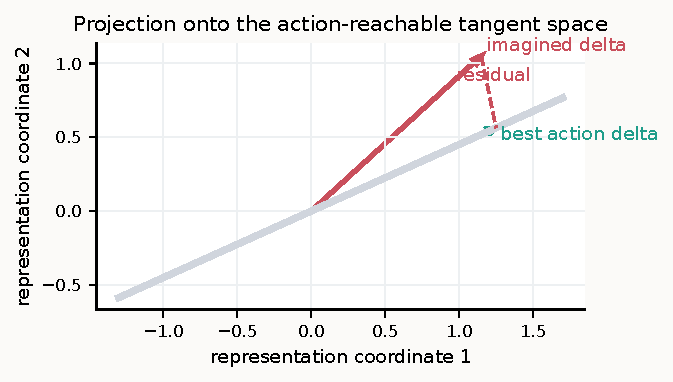
\includegraphics[width=0.45\linewidth]{figures/fig2_geometry_projection.pdf}
\caption{A generated future can be visually plausible while leaving the local action-reachable tangent set. The actionability residual projects an imagined representation change onto $\operatorname{Im}(J_\phi)$ under action limits and penalizes the residual.}
\label{fig:concept}
\end{figure}
